
\setcounter{section}{0}
\setcounter{figure}{0}
\graphicspath{{./figs/}{./figs/item-jingtong/}}

\NewsTitle{Accumulative Computing: Sensing With Unlimited Free Energy}
\NewsAuthor{Jingtong Hu, Oklahoma State University}

\section{Introduction and Motivation}

Sensors are an integral part of Cyber-Physical Systems (CPS).  
While battery and cable power are still the major energy source for many sensors, there is a class of devices in which it is challenging to employ battery or cable power since it is inconvenient, costly or even dangerous to replace or service them. Examples of such applications include implantable sensor, wearable health monitor, water pipeline or building HVAC status monitor, soil or water pollution monitor, etc.
Energy harvesting techniques, which generate electric energy from their ambient environment using direct energy conversion techniques, are very attractive to these applications because they can eliminate
the need for batteries or wires and enable long-term adoption of these systems.

\begin{wrapfigure}{R}{0.45\linewidth} 
\vspace{-25pt}
\centering
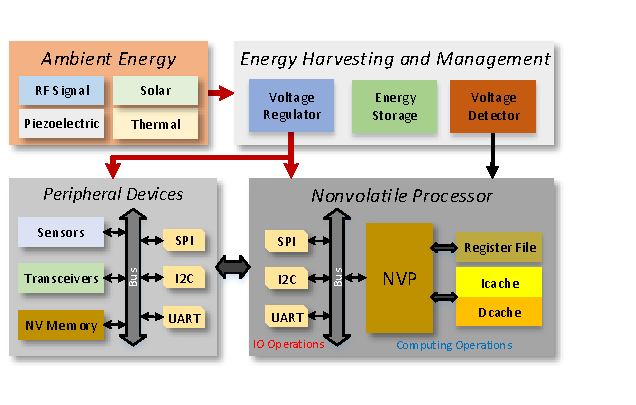
\includegraphics[width=.5\textwidth]{system_architecture.pdf}
\vspace{-35pt}
\caption{Energy Harvesting System}
\label{fig:sys}
\vspace{-6pt}
\end{wrapfigure}

Figure~\ref{fig:sys} shows the architecture for a typical energy harvesting based sensing system.
%Energy harvesting devices generate electric energy from their ambient environment using direct energy conversion techniques. 
Ambient energy such as light, kinetic, RF, thermal, or even biochemical energy, are harvested and stored in a small capacitor, which can be used to power the processor and peripheral devices with on-chip converters~\cite{Tida:2014:NTI:2686762.2637481}. However, there is an intrinsic drawback with harvested energy sources. They are \textbf{intermittent}. Since almost all traditional computer systems are designed based on the assumption of a stable power supply, none of them can make significant progress under frequently interrupted power. In order to take advantage of unlimited free energy supply, a new computing paradigm which can make progress even under intermittent power is needed.

%What is worse, large tasks could possibly never finish since the intermediate results cannot be saved. 
%With an unstable power supply, the whole computer system will be interrupted frequently, which will cause severe performance degradation. 

In order to make progress, we have to \textbf{accumulate} the computing across intermittent power cycles. The key idea is to save the processor's volatile registers to a non-volatile memory (NVM) when there is a power failure and restore the processor state when the power comes back on. There have been several works to achieve this with either software assisted approach~\cite{6960060,Jayakumar:2015:QUR:2810396.2700249,Ransford:2011:MSS:1950365.1950386} or hardware approach~\cite{7056060}. While existing research shows exciting advancement, there are still challenges that need to be answered to make self-powered accumulative computing a mature platform. 

%NVMs, which can retain data even when the power is off, are natural candidates to save processor state during power failure. 
%
%In order to achieve better register checkpointing and system performance, the PI has developed several compiler optimization techniques, including non-volatile register aware instruction scheduling and energy aware checkpointing position selection~\cite{DBLP:conf/rtcsa/XiePHXZ14,DBLP:conf/aspdac/XiePHYC15,Zhao:2015:SAN:2755753.2755881}. Based on these preliminary works, the PI was awarded an NSF CISE CRII grant to work on \textbf{register} level code optimization for the Non-volatile Processor (NVP). With the support, the PI has further devised inconsistency elimination, stack trimming, and energy aware scheduling~\cite{DBLP:conf/dac/XieZPHLX15,Li:2015:CDA:2744769.2744809,Li:2016:PTS:2897937.2898059} to ensure the correctness and efficiency of programs executing on NVP.  

% , with either software assisted approach~\cite{Ransford:2011:MSS:1950365.1950386,6960060,Jayakumar:2015:QUR:2810396.2700249} or hardware approach~\cite{7056060}.  ~\cite{7059068,1609379,5542984,PIZ09}


\begin{itemize}[noitemsep,topsep=0pt,parsep=0pt,partopsep=0pt]
\item First, while most existing works are successful in achieving the continuous computing functionality, few of them considered optimizing the checkpointing efficiency. On one hand, the energy harvested in such systems is usually limited. On the other hand, not only registers need to be checkpointed, but on-chip and off-chip memories also need to be checkpointed if they are volatile. Therefore, fast and efficient checkpointing is needed for the whole volatile memory hierarchy to ensure successful checkpointing. Meanwhile, more energy can be used for system forward progress.
\item Second, while the computing status can be saved, I/O interfaces associated with peripheral sensors and communication devices are hard to checkpoint due to their time-sensitivity and atomicity. In many cases, interrupted operations need to be restarted from the beginning, which will severely affect the forward progress. Meanwhile, checkpointing for processor and I/O operations in interrupt service routines (ISRs) has to be handled properly to ensure correct execution.
\item Third, when multiple tasks are running concurrently in the system, the OS scheduler and task management will also affect the forward progress upon power failure. 
\item  Additionally, our study~\cite{DBLP:conf/dac/XieZPHLX15} showed that without considering the volatility across the memory hierarchy, data inconsistency might happen and lead to fatal errors. 
\end{itemize}

\section{Checkpoint Efficiency Optimization}
Several works have been done to optimize the checkpoint efficiency. First, we have developed a stack trimming technique to minimize stack data that need to be checkpointed~\cite{Li:2015:CDA:2744769.2744809}. The idea is to reduce the stack size via address space sharing. Within a program, each function instance is associated with a \textit{frame} (also called \textit{active record}) to store the context information for this function. Local data, including local variables and compilation temporary variables, are stored in this frame. A conventional stack based allocator works as follows: a specific memory address is assigned to the \textit{main} function's frame. When a function is called, the callee function's frame is allocated on top of the caller function's frame. When a function returns, the callee function's frame is deallocated from the top of caller function's frame.
Traditionally, the stack space is separately allocated for the caller and callee functions, which is conservative and results in a large stack size. 
%In this work, we propose a novel stack allocation scheme for stack trimming through address space sharing.


\begin{figure*}[htbp!]
\centering
\begin{minipage}{0.3\linewidth}
\centering
%\resizebox{!}{!}{
%\ProgramSurround
%\InBodyLeftNumberLine
\begin{spacing}{0.5}
\begin{program}  
struct T
\{
	int i;
	int j;
	char arr[10];
\};

int cpyT( T *t1, *t2 )
\{
	int a;
	int b;		
	modify(\&a);	
	t1.i = t2.i + a;
	modify(\&b);
	t1.j = t2.j + b;	
	strcpy(t1.arr, t2.arr);		
	return 0;
\}
\end{program}
\end{spacing}
\vspace{-.2in}
\caption{An example program} %For simplicity, the code of function \textit{modify} and \textit{strcpy} is not listed here.
\label{fig:sampleCode}
\end{minipage}
%\hspace{0.35in}
\begin{minipage}{0.6\linewidth}
\centering
\vspace{.35in}
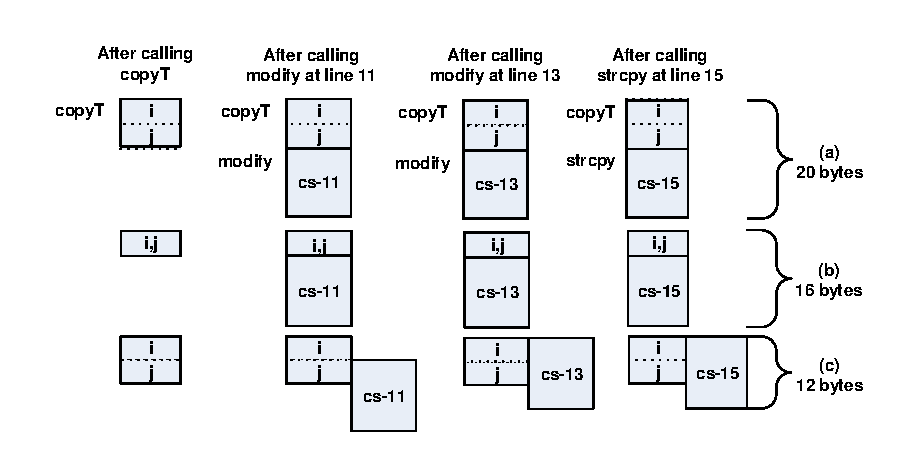
\includegraphics[width=\textwidth]{stackSizeMoti.pdf}
%\vspace{.15in}
\caption{Comparison of stack size under different stack allocation schemes. Assume that the frame size of \textit{copyT}, \textit{modify} and \textit{strcpy} is 8, 4 and 12 bytes, respectively.}
\label{fig:stackSizeMoti}
\end{minipage}
\end{figure*}




%\vspace{-.4in}
% (a) The conventional allocation scheme. (b) The allocation scheme with data overlaying among data objects. (c) The allocation scheme with data overlaying among data objects and call sites.
%\includegraphics[width=\textwidth]{figs/examplecode2.eps}
%examplecode2.eps
A simple motivation example is presented to illustrate how stack allocation schemes affect the stack size.
The example code is shown in Figure \ref{fig:sampleCode}.
%The \textit{live range} for each local object of function \textit{copyT} is shown in Figure \ref{fig:liveRangeMoti}.
Note that each call site (cs) is also viewed as a local object, and its size is equal to the callee function's frame size. Figure \ref{fig:stackSizeMoti} illustrates the stack size under different schemes.
Figure \ref{fig:stackSizeMoti}(a) shows that the conventional allocation scheme, without any overlay in stack, holds the largest stack size of 20 bytes. Since \textit{i} and \textit{j} have disjoint live ranges, they can be coalesced. The result is shown in 
Figure \ref{fig:stackSizeMoti}(b). Here, the frame size of \textit{copyT} is reduced by 4 bytes, and the maximum stack size is reduced to 16 bytes. In order to further reduce stack size, we aggressively overlay call sites with disjoint live ranges~\cite{Li:2015:CDA:2744769.2744809}. Figure \ref{fig:stackSizeMoti}(c) shows the result, in which the maximum stack size can be reduced to 12 bytes. From this example, we can see that objects with disjoint live ranges can share the same address without violating the data integrity and thus reduce the stack size. The experimental results show that the proposed technique can reduce the stack size by 28.6\% on average for a wide range of benchmarks. 


\begin{figure}[htbp]
\centering
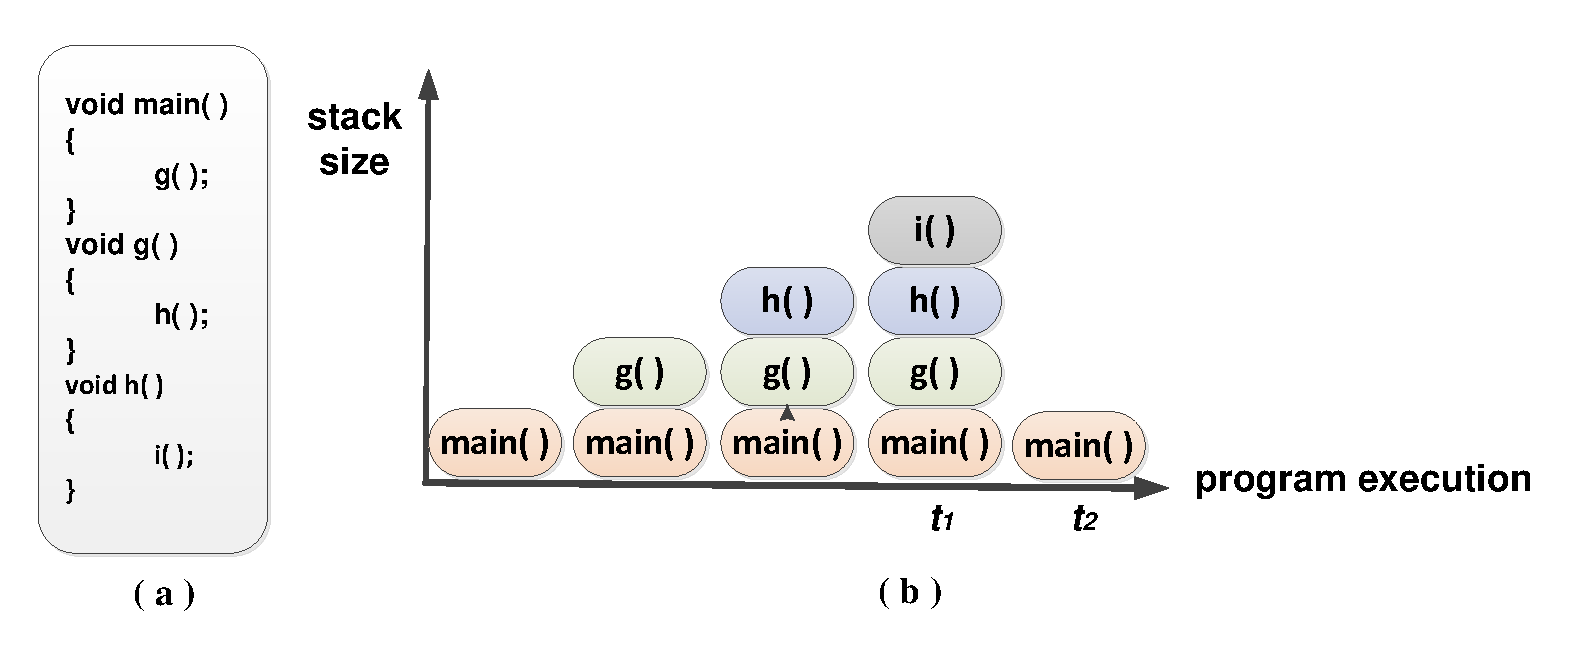
\includegraphics[width=.5\textwidth]{motivation0917_stack.pdf}
   \caption{Stack Fluctuation.}
   \label{fig:motviation}
\end{figure}


In addition to the stack trimming, there are also optimization opportunities in the temporal domain. Figure~\ref{fig:motviation}(a) shows an example code, where the \textit{main} function invokes function \textit{g}; \textit{g} invokes \textit{h}; and \textit{h} invokes \textit{i}. The stack usage is shown in Fig. \ref{fig:motviation}(b). From the figure, we can see that the stack size fluctuates as the functions are invoked and return. Assume that the system detects power failure at time \textit{$t_1$}. The conventional backup strategy is \textit{instant backup}, where all the processor states are backed up immediately at \textit{$t_1$}. In this case, this system needs to checkpoint four stack frames. However, instead of consuming a large portion of remaining energy to checkpoint, we can spend some energy to continue the program execution until \textit{$t_2$}. At \textit{$t_2$}, there is only one stack frame to checkpoint since all the callees already returned. Based on this observation, we developed a three-step approach~\cite{Zhao:2015:SAN:2755753.2755881}, in which the best backup positions are derived in polynomial time. The evaluation results show considerable checkpoint content reduction compared with instant checkpoint.

\section{Conclusion}
Realizing accumulative computing on unstable harvested energy will enable a new class of self-powered sensing/monitoring systems that can last for years and require the least maintenance effort in various non-timing critical applications. It will simplify system installation and maintenance in many areas such as health care, building monitoring and maintenance, traffic, agriculture and environment monitoring, and even crisis management. Meanwhile, it will help bridge the gap between ever-increasing electronic power needs and battery scalability and have the potential to provide a large infrastructure for opportunistic computing with great social impact. However, there all still several challenges to be answered to achieve the goal. This article presents two checkpoint efficiency optimization techniques which aim to overcome these challenges.

\bibliographystyle{plain}
\bibliographystyle{abbrv}
%\bibliography{ref,NVP}
\begin{thebibliography}{1}

\bibitem{6960060}
D.~Balsamo, A.~S. Weddell, G.~V. Merrett, B.~M. Al-Hashimi, D.~Brunelli, and
  L.~Benini.
\newblock Hibernus: Sustaining computation during intermittent supply for
  energy-harvesting systems.
\newblock {\em IEEE Embedded Systems Letters}, 7(1):15--18, March 2015.

\bibitem{Jayakumar:2015:QUR:2810396.2700249}
Hrishikesh Jayakumar, Arnab Raha, Woo~Suk Lee, and Vijay Raghunathan.
\newblock Quickrecall: A hw/sw approach for computing across power cycles in
  transiently powered computers.
\newblock {\em J. Emerg. Technol. Comput. Syst.}, 12(1):8:1--8:19, August 2015.

\bibitem{Li:2015:CDA:2744769.2744809}
Qingan Li, Mengying Zhao, Jingtong Hu, Yongpan Liu, Yanxiang He, and Chun~Jason
  Xue.
\newblock Compiler directed automatic stack trimming for efficient non-volatile
  processors.
\newblock In {\em Proceedings of the 52nd Annual Design Automation Conference},
  DAC '15, pages 183:1--183:6, 2015.

\bibitem{7056060}
K.~Ma, Y.~Zheng, S.~Li, K.~Swaminathan, X.~Li, Y.~Liu, J.~Sampson, Y.~Xie, and
  V.~Narayanan.
\newblock Architecture exploration for ambient energy harvesting nonvolatile
  processors.
\newblock In {\em 2015 IEEE 21st International Symposium on High Performance
  Computer Architecture (HPCA)}, pages 526--537, Feb 2015.

\bibitem{Ransford:2011:MSS:1950365.1950386}
Benjamin Ransford, Jacob Sorber, and Kevin Fu.
\newblock Mementos: System support for long-running computation on rfid-scale
  devices.
\newblock In {\em Proceedings of the Sixteenth International Conference on
  Architectural Support for Programming Languages and Operating Systems},
  ASPLOS XVI, pages 159--170, 2011.

\bibitem{Tida:2014:NTI:2686762.2637481}
Umamaheswara~Rao Tida, Cheng Zhuo, and Yiyu Shi.
\newblock Novel through-silicon-via inductor-based on-chip dc-dc converter
  designs in 3d ics.
\newblock {\em J. Emerg. Technol. Comput. Syst.}, 11(2):16:1--16:14, November
  2014.

\bibitem{DBLP:conf/dac/XieZPHLX15}
Mimi Xie, Mengying Zhao, Chen Pan, Jingtong Hu, Yongpan Liu, and Chun~Jason
  Xue.
\newblock Fixing the broken time machine: consistency-aware checkpointing for
  energy harvesting powered non-volatile processor.
\newblock In {\em Proceedings of the 52nd Annual Design Automation Conference},
  pages 184:1--184:6, 2015.

\bibitem{Zhao:2015:SAN:2755753.2755881}
Mengying Zhao, Qingan Li, Mimi Xie, Yongpan Liu, Jingtong Hu, and Chun~Jason
  Xue.
\newblock Software assisted non-volatile register reduction for energy
  harvesting based cyber-physical system.
\newblock In {\em Proceedings of the 2015 Design, Automation \& Test in Europe
  Conference \& Exhibition}, DATE, pages 567--572, 2015.

\end{thebibliography}
